\documentclass[compress]{beamer}

\mode<presentation> {
\usetheme{Luebeck}
\hypersetup{pdfpagemode=FullScreen}
\setbeamertemplate{footline}[frame number] % To replace the footer line in all slides with a simple slide count uncomment this line
\setbeamertemplate{headline}[default]
\setbeamertemplate{navigation symbols}{}
\setbeamertemplate{caption}[numbered]

% define your own colors:
\definecolor{gold}{rgb}{260,195,0}
%\definecolor{GTgold}{cmyk}{0,0.241,0.933,0.122}
\definecolor{KFUPMgreen}{cmyk}{0.756,0,0.756,0.196}

% Make GT-CSIP footer logo scheme
\setbeamercolor{structure}{fg = KFUPMgreen,bg=blue!40!gold}
%\setbeamercolor{structure}{fg =KFUPMgreen, bg=GTgold}
\setbeamercolor*{palette primary}{use=structure,fg=white,bg=blue!40!gold}
}

% Packages
\usepackage[utf8]{inputenc}
\usepackage[english]{babel}
\usepackage{mathtools}
\usepackage{graphicx}
\graphicspath{{fig/}}
\usepackage{color}
\usepackage{listings}
\usepackage[]{mcode}
\usepackage{hyperref}
\hypersetup{
    colorlinks=true,
    linkcolor=blue,
    filecolor=magenta,      
    urlcolor=cyan,
}

\urlstyle{same}

\newcommand{\CC}{C\nolinebreak\hspace{-.05em}\raisebox{.4ex}{\tiny\bf +}\nolinebreak\hspace{-.10em}\raisebox{.4ex}{\tiny\bf +}}

% Title
\titlegraphic{
\includegraphics[width=4cm]{Leftlogo}\hspace*{4.75cm}~%
   
\includegraphics[width=2.5cm]{CeGPlogo}
}
\title{Python\textsuperscript{\texttrademark} vs. MATLAB\textsuperscript{\textregistered} in Scientific Computing}
\author[shortname]{Lijun Zhu}
\institute{CeGP, Georgia Tech}
\date{\today}

%  Outline at each section
\AtBeginSection[] {
  \begin{frame}
   \frametitle{Outline}
    \tableofcontents[currentsection]
    \addtocounter{framenumber}{-1}
  \end{frame}
}

\begin{document}

\begin{frame}[noframenumbering,plain]
\titlepage
\end{frame}

\setcounter{framenumber}{0}

\begin{frame}
\frametitle{Outline}
\tableofcontents
\end{frame}

\begin{frame}
	\frametitle{Disclaimers}
	\begin{itemize}
		\item This sets of slides serves as an introduction to Python in scientific copmuting
		\item It is not intended to be a tutorial
		\item Many of the contents are subjective
		\item Useful info/webpages are given at the end of the presentation for future reference
		\item If interested, I can give a tutorial on any specific area
	\end{itemize}
\end{frame}

\section{Motivation}
\begin{frame}
	\frametitle{Motivation: a real-life scenario}
	\begin{itemize}
		\item Seismic signal processing tasks
		\begin{itemize}
			\item Download data from online data center
			\item Process and plot the target data
			\item Document code/algorithm for future reference	
			\item Save data and collaborate with others
		\end{itemize}
		\item What I am looking for
		\begin{itemize}
			\item Effortless data input/output
			\item Easy and intuitive way to try some candidate algorithms
			\item Generate great looking plots
			\item Standard packaging and online user support
			\item Good to transfer data and collaborate with other researchers 
		\end{itemize}
	\end{itemize}
\end{frame}

\begin{frame}
	\frametitle{MATLAB\textsuperscript{\textregistered} only solution}
	\begin{itemize}
		\item Download dataset/station info from IRIS website
		\item Manually convert those info into MATLAB structure and use irisFetch.m to fetch data (Tedious)
		\item Process data and generate plots (\href{http://www.crewes.org/ResearchLinks/FreeSoftware/}{plotseis}, \href{http://www.mathworks.com/matlabcentral/fileexchange/38691-wiggle}{wiggle} etc.)
		\item Improve plots for publishing (\href{http://www.mathworks.com/matlabcentral/fileexchange/34055-tightfig}{tightfig}, \href{http://www.mathworks.com/matlabcentral/fileexchange/27991-tight-subplot-nh--nw--gap--marg-h--marg-w-}{tight\_subplot} etc.)
			\item Document code by MATLAB built-in docs and publish on personal website
		\item Save data in .MAT (later convert to other format such as .SAC, .SEGY, .SU using other third-party packages)
	\end{itemize}
\end{frame}

\begin{frame}
	\frametitle{Mix MATLAB\textsuperscript{\textregistered} with other tools}
	\begin{itemize}
		\item Download dataset/station info from IRIS website
		\item Use AWK on UN*X system to generate a email template sent to IRIS serve
		\item Download data in .SEED format by FTP link from IRIS server
		\item Use SAC to convert .SEED to .SAC files
		\item Use \href{http://geophysics.eas.gatech.edu/people/zpeng/Teaching/SAC_Tutorial/\#part2_6}{MatSAC} in MATLAB to load .SAC files
		\item Process data and generate plots in PNG/PDF format
		\item Post-process image to merge/modify plots into good appearance (\href{http://www.adobe.com/products/illustrator.html}{Adobe Illustrator} etc.)
		\item Document code by Latex generated PDF files/REAMME.me
		\item Save data in .MAT (later convert to other format such as .SAC, .SEGY, .SU using other third-party packages)
	\end{itemize}
\end{frame}

\begin{frame}
	\frametitle{Python\textsuperscript{\texttrademark} solution}
	\begin{itemize}
		\item Download dataset/station info from IRIS website and save in txt file
		\item Automatically(regular expression) load txt file into python and use \href{https://github.com/obspy/obspy/wiki}{ObsPy} to request data from IRIS database (Easier)
		\item Process data by \href{http://www.numpy.org/}{NumPy} and \href{http://scipy.org/}{SciPy}, then generate plots by \href{http://matplotlib.org/}{Matplotlib}
		\item Improve plots by \href{http://www.pyqtgraph.org/}{PyQtGraph} etc.
		\item Document code by \href{http://www.sphinx-doc.org/en/stable/}{Sphinx} and publish code in \href{https://pypi.python.org/pypi}{PyPI} which is downloadable through \href{https://pip.pypa.io/en/stable/}{pip}
		\item Save data in the format that will be used to collaborate with others
	\end{itemize}
\end{frame}

\begin{frame}
	\frametitle{Summary: a real-life scenario}
	\begin{itemize}
		\item MATLAB\textsuperscript{\textregistered} only solution
		\begin{itemize}
			\item \textcolor{red}{Unified} development environment ($+$)
			\item \textcolor{red}{Optimized} for matrix operation and linear algebra with little effort required ($+$)
			\item \textcolor{red}{Not ideal} for some task (e.g. string manipulation) ($-$)
			\item \textcolor{red}{Limited} to MATLAB tools ($-$)
		\end{itemize}
		\item Mix MATLAB\textsuperscript{\textregistered} with other tools
		\begin{itemize}
			\item Use the \textcolor{red}{right tool} for the right task ($+$)
			\item \textcolor{red}{Full potential} of optimization ($+$)
			\item \textcolor{red}{De-centralized} development environment and difficult to package ($-$)
		\end{itemize}
		\item Python\textsuperscript{\texttrademark} solution
		\begin{itemize}
			\item \textcolor{red}{Unified} development environment and packaging system for publishing code online
			\item \textcolor{red}{Full potential} of optimization with \textcolor{red}{incremental} effort requirement
		\end{itemize}
	\end{itemize}
\end{frame}

\section{Python\textsuperscript{\texttrademark} vs. MATLAB \textsuperscript{\textregistered}}
\begin{frame}
	\frametitle{Python\textsuperscript{\texttrademark} vs. MATLAB \textsuperscript{\textregistered}}
	\centering
	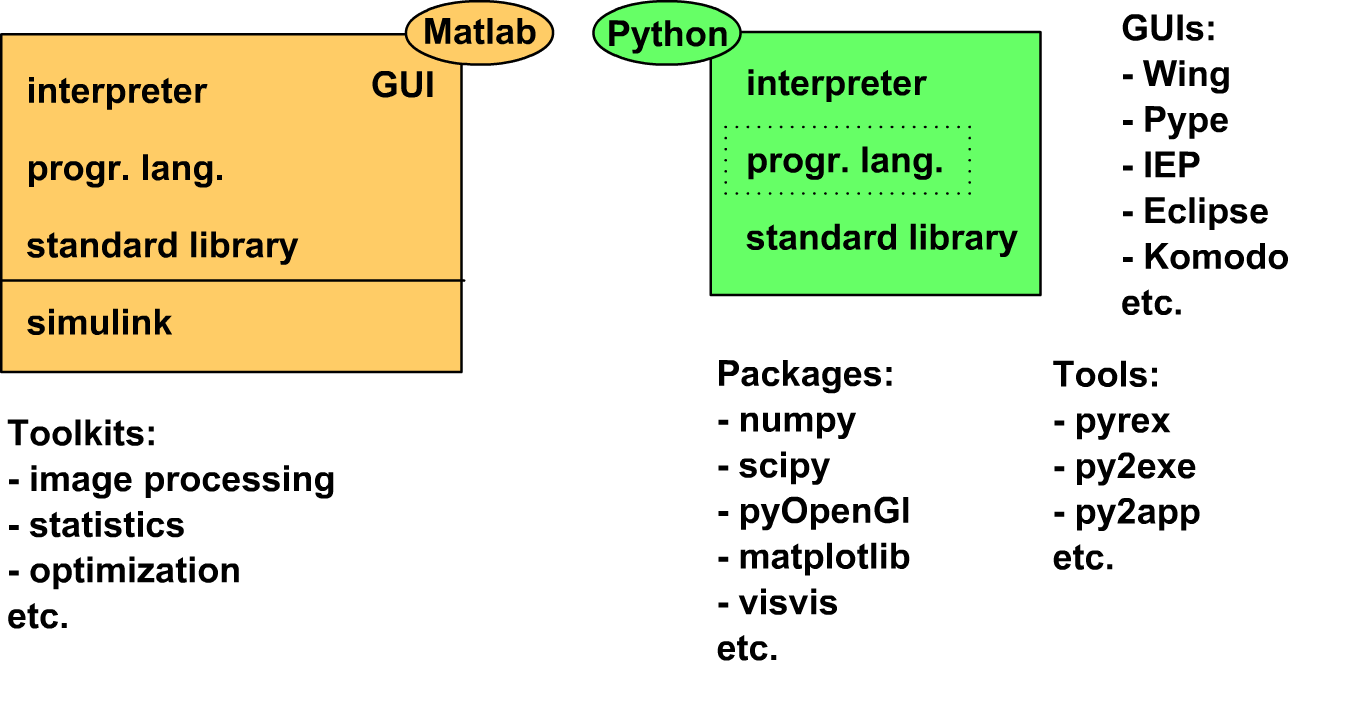
\includegraphics[width=\textwidth]{fig/pythonVSmatlab}
\end{frame}

\subsection{Functionality and features}
\begin{frame}
	\frametitle{Features comparison}
	\begin{table}
		\caption{Basic and expendable feature comparison between MATLAB and Python}
		\begin{tabular}{|l|c|c|}
			\hline
			Features			& 	MATLAB 		& 	Python\\\hline		
			Interactive console	&	Built-in 	& 	IPython\\\hline
			IDE					&	Built-in	&	Sublime Text, Komodo, \href{https://wiki.python.org/moin/IntegratedDevelopmentEnvironments}{etc.}\\\hline	
			Matrix operation	&	Built-in	& 	Numpy\\\hline
			Linear algebra		&	Built-in	&	Scipy\\\hline
			Plotting			& 	Built-in	&	Matplotlib\\\hline
			Signal Processing	&	Toolbox		&	Scipy\\\hline
			Optimization		&	Toolbox		&	Scipy\\\hline
			Statistics			&	Toolbox		&	Pandas\\\hline
			Symbolic Math 		&	Toolbox		&	Sympy\\\hline
			Expansion			&	C/\CC, Fortran	&	C/\CC, Fortran, R etc$^\dagger$.\\\hline
		\end{tabular}
	\end{table}
	\begin{itemize}
		\tiny \item $\dagger$: Python can be a wrapper for packages written in most other languages (Even MATLAB)
	\end{itemize}
\end{frame}

\begin{frame}
	\frametitle{Interactive console}
	\begin{itemize}
		\item MATLAB
		\begin{figure}
			\centering
			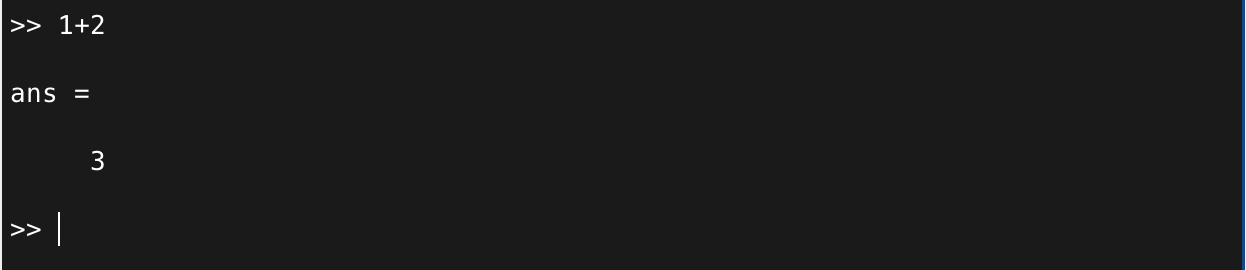
\includegraphics[width=\linewidth]{fig/matlab_console}
		\end{figure}
		\item Python
				\begin{figure}
			\centering
			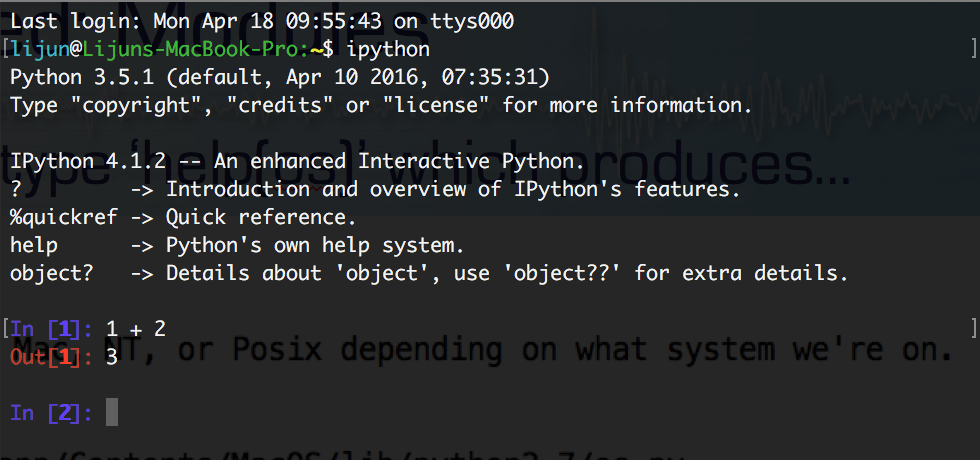
\includegraphics[width=\linewidth]{fig/ipython}
		\end{figure}
	\end{itemize}
\end{frame}

\begin{frame}
	\frametitle{Integrated Development Environments(IDE): MATLAB}
	\begin{itemize}
		\item Good UI and effective profiler
		\item Integrator console and file browser
	\end{itemize}
	\begin{figure}
		\centering
		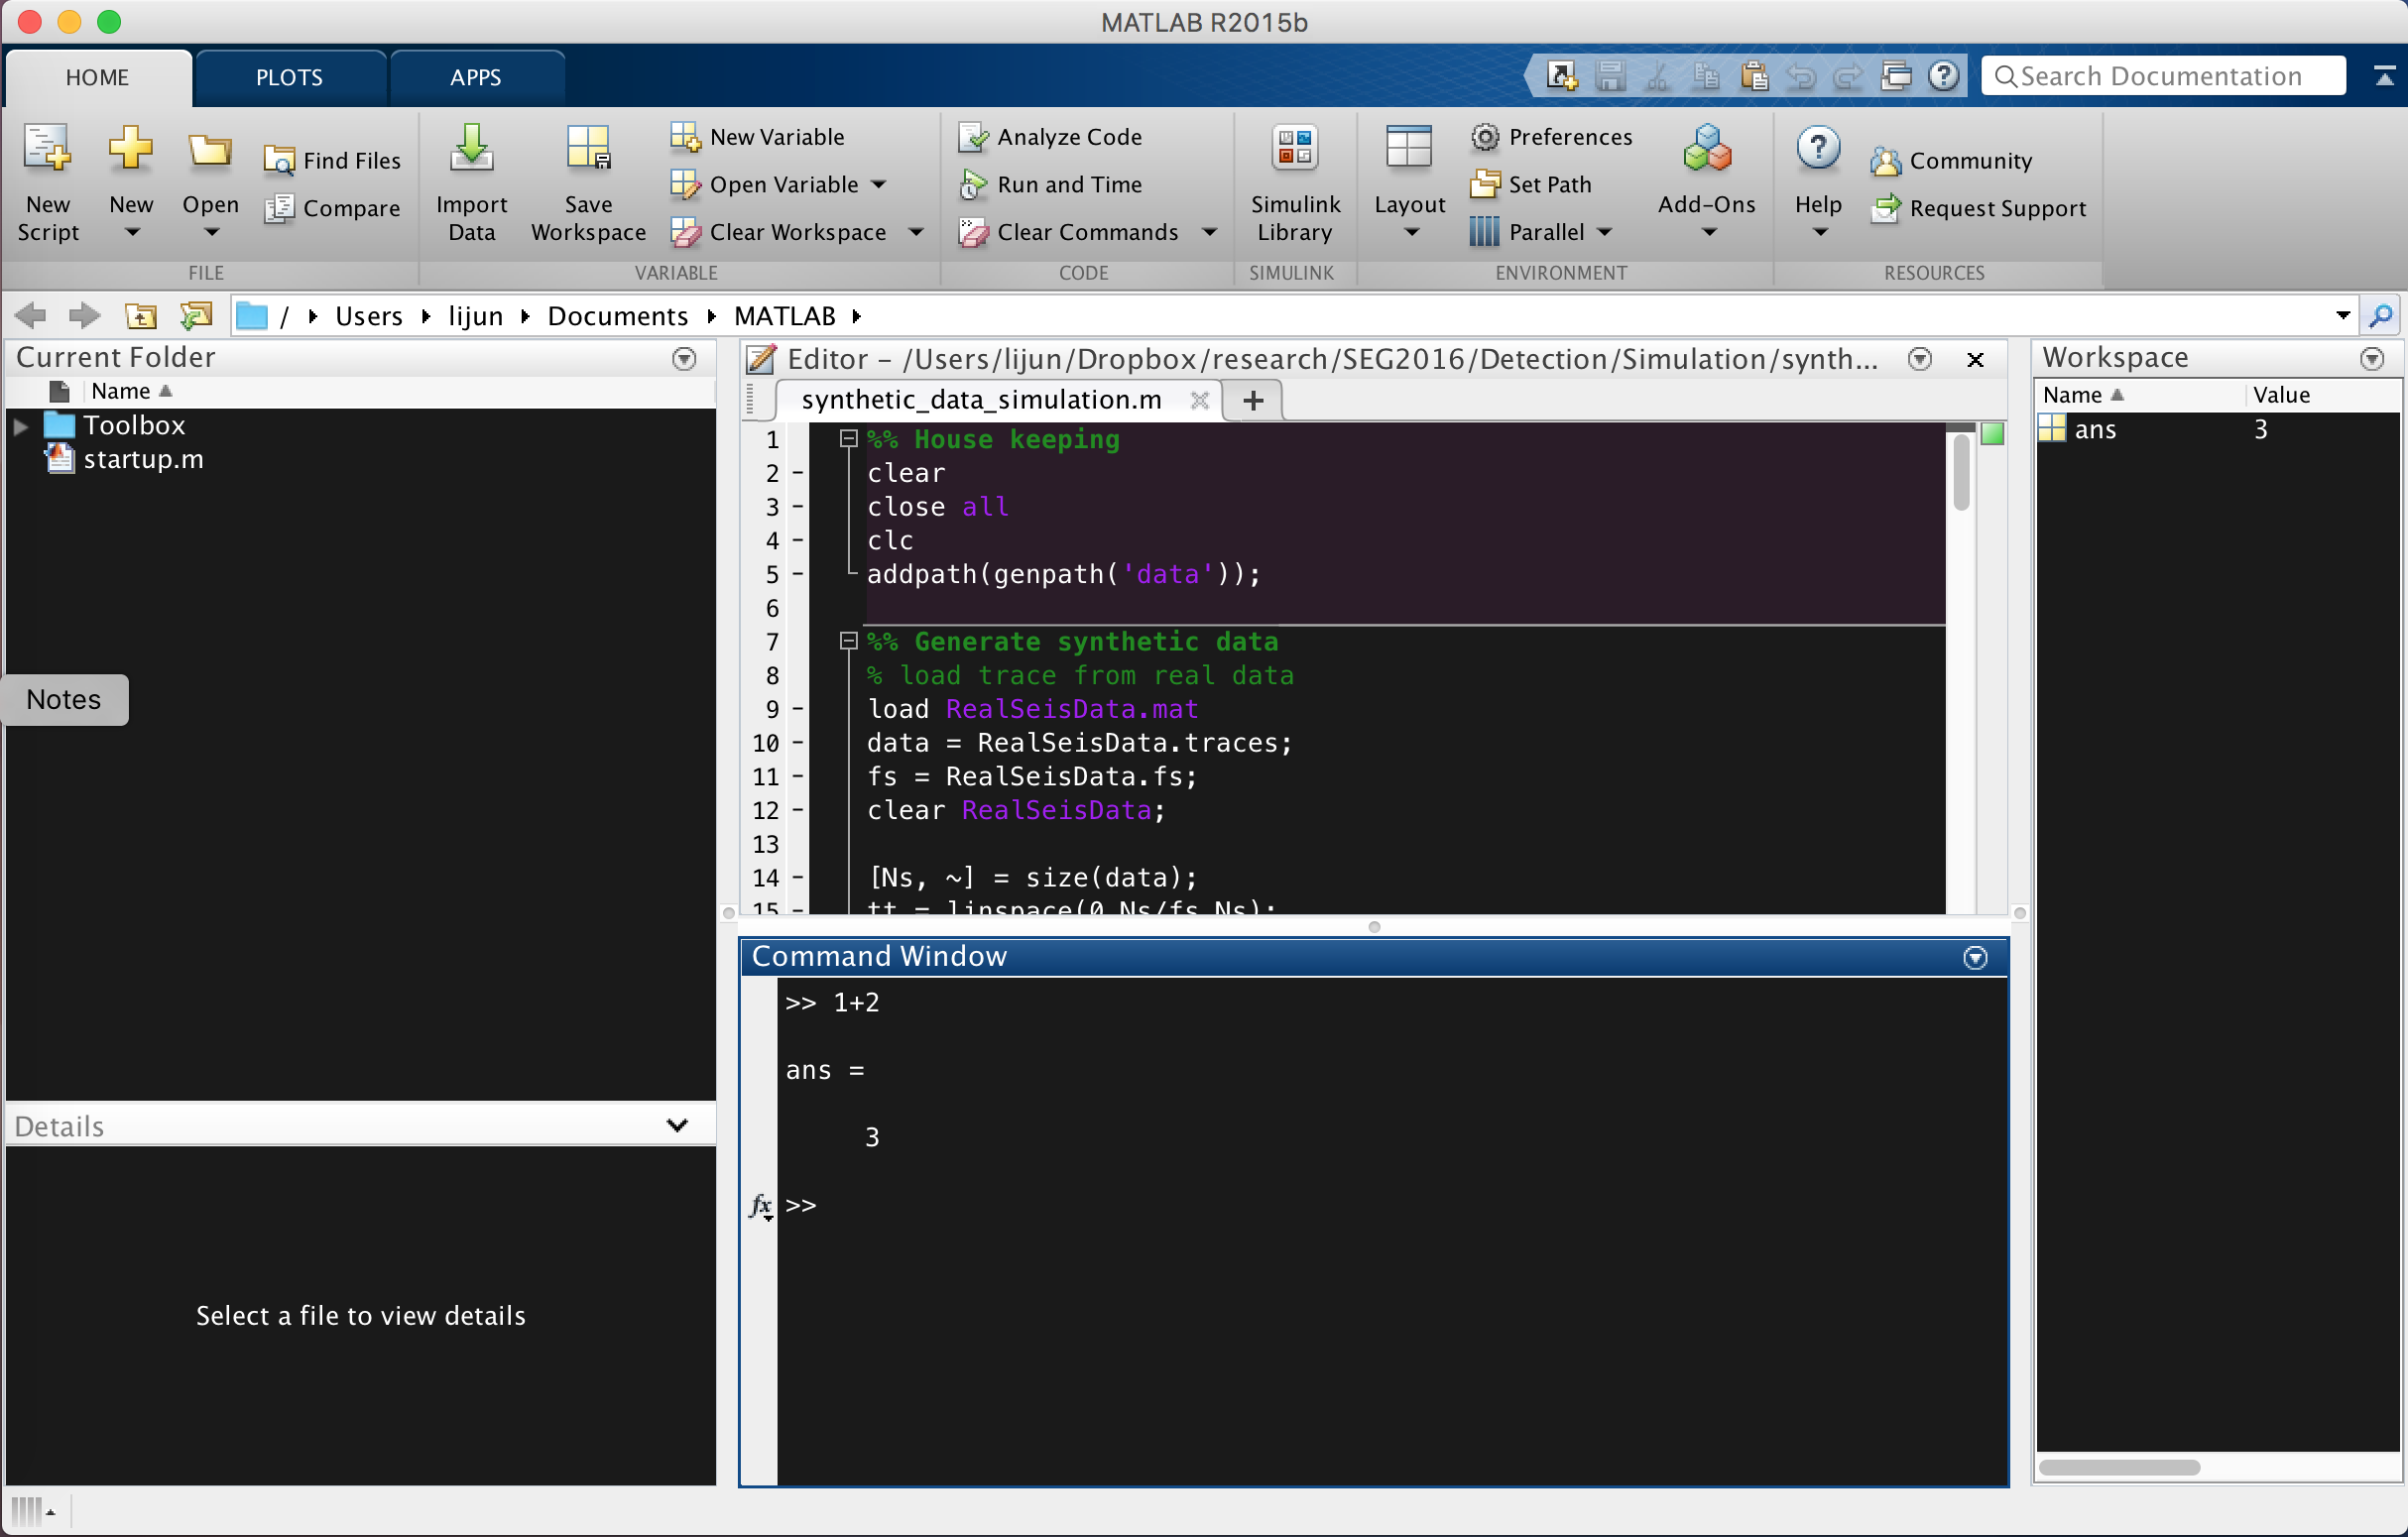
\includegraphics[width=\textwidth]{fig/matlabIDE}
	\end{figure}
\end{frame}

\begin{frame}
	\frametitle{Python: Sublime Text + Anaconda addon}
	\begin{itemize}
		\item Nice and clean UI with most needed functonality
		\item Lack of a good profiler
	\end{itemize}
	\begin{figure}
		\centering
		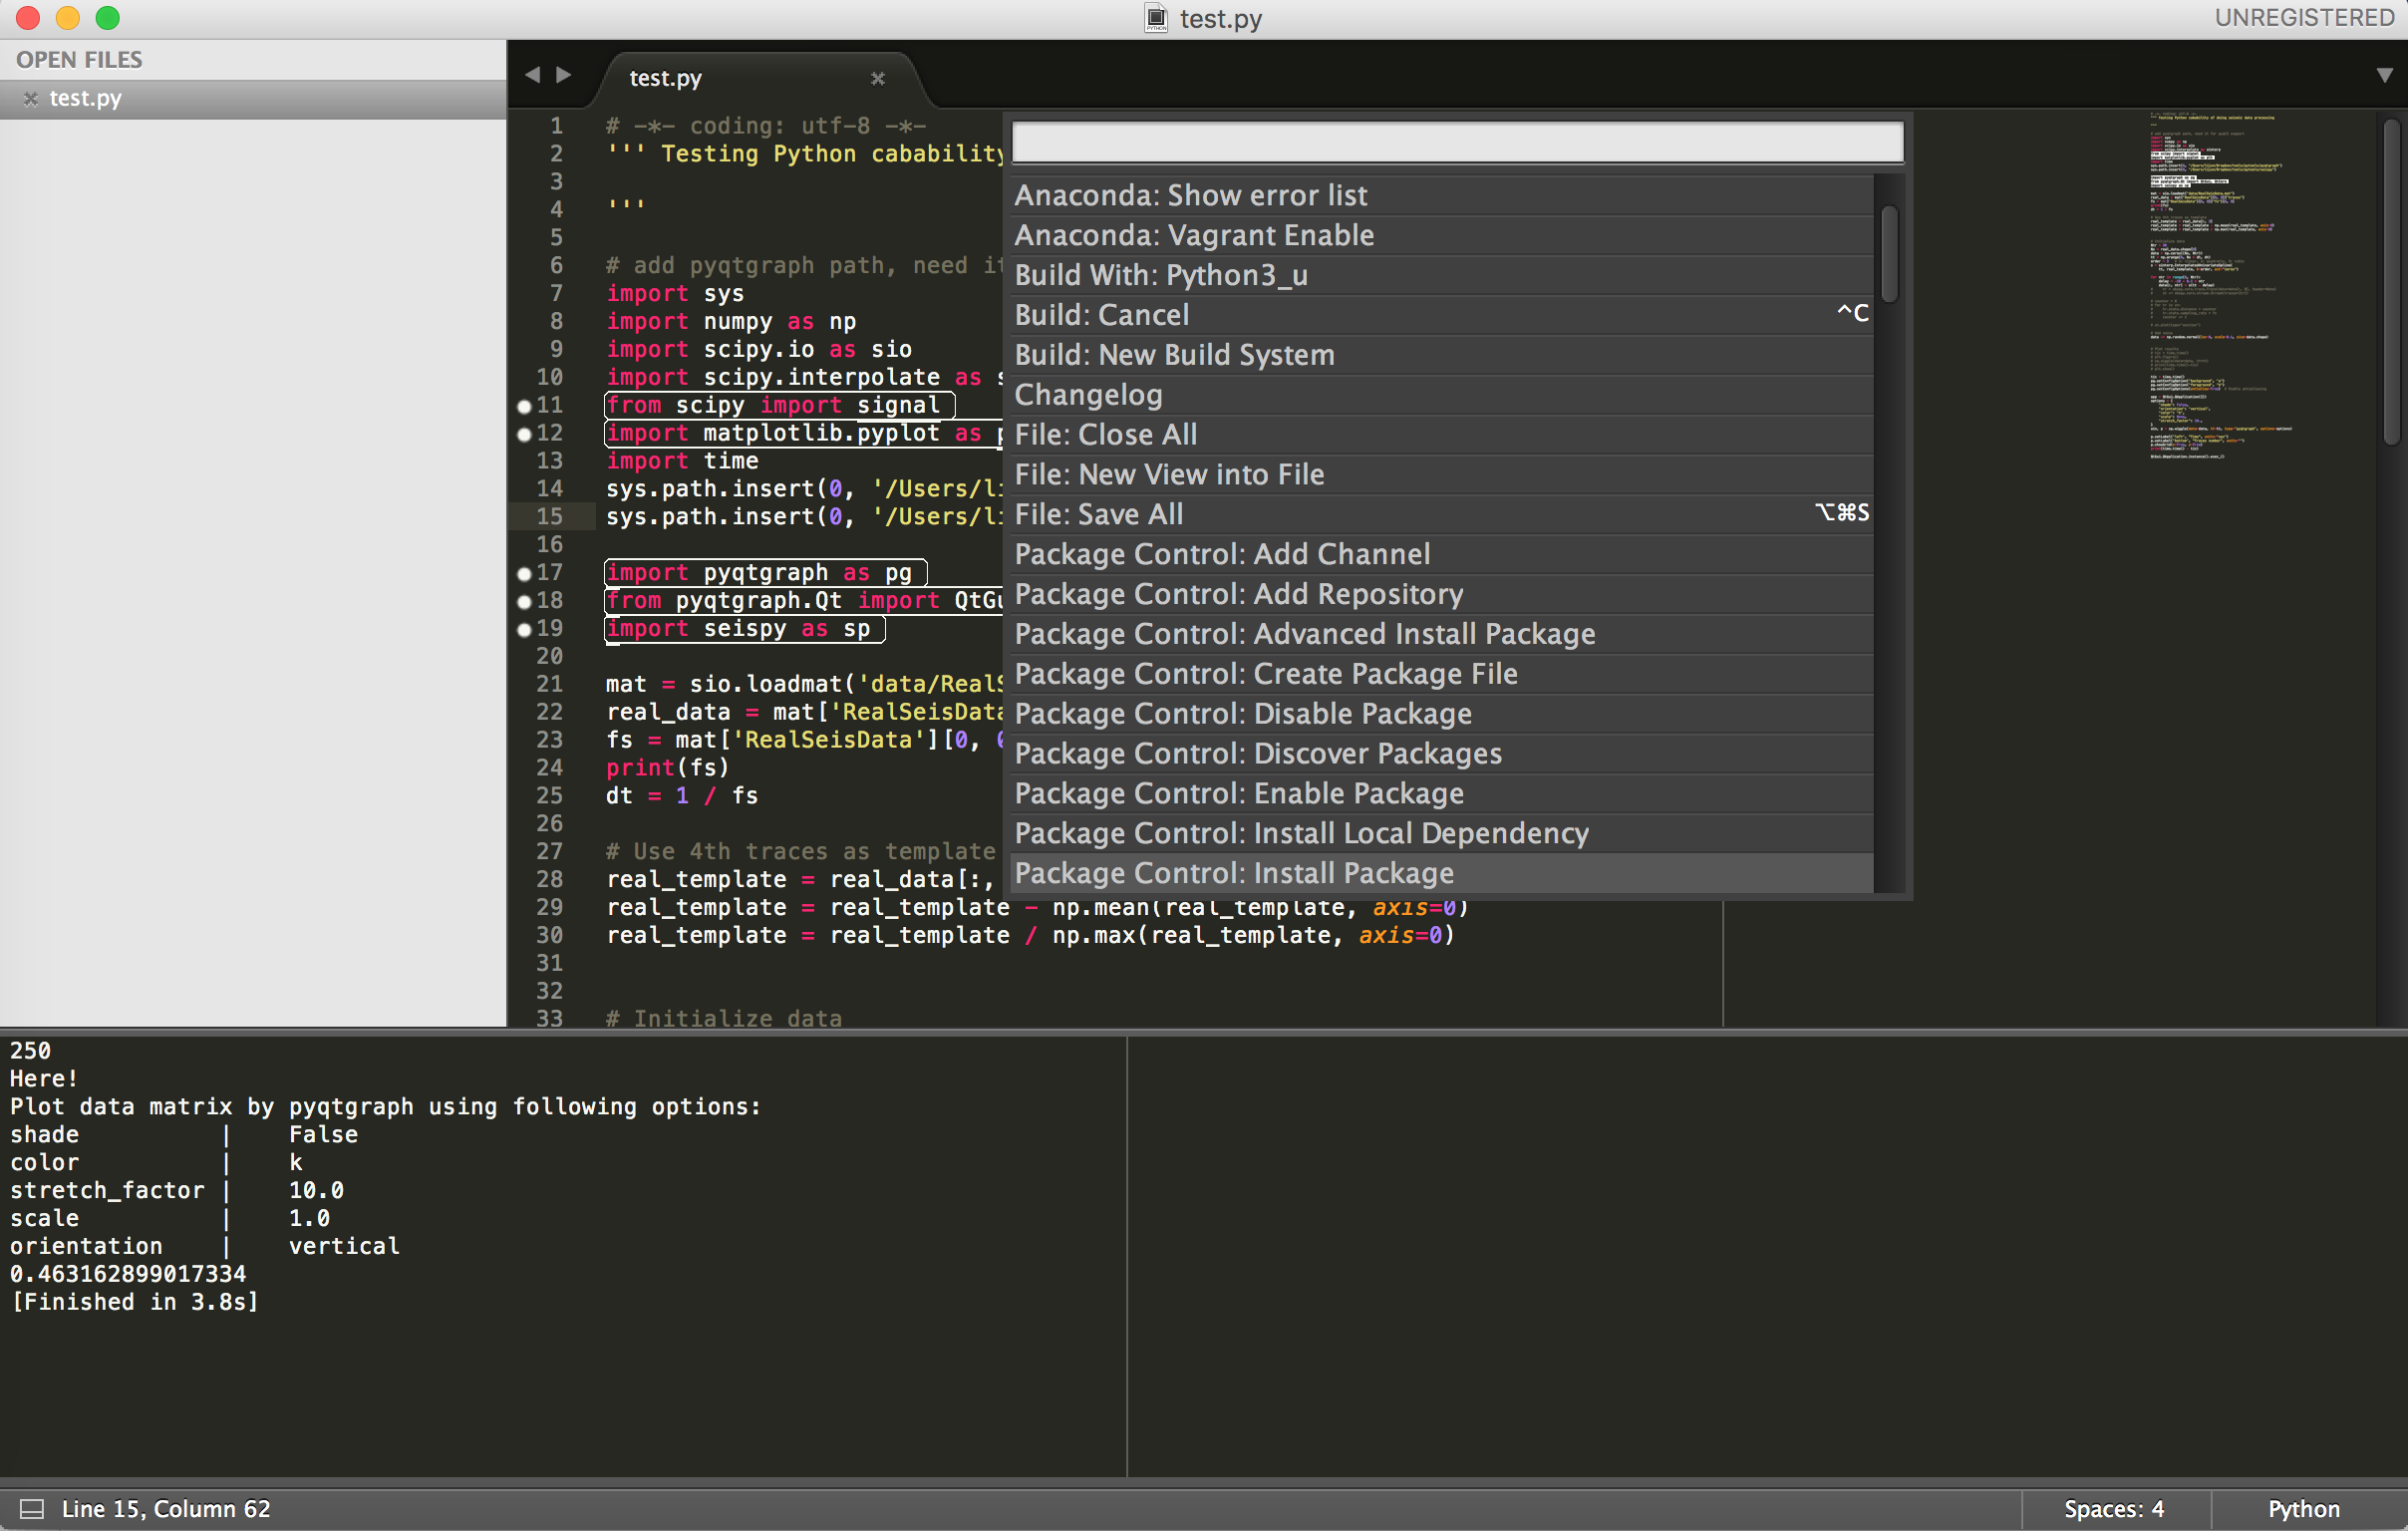
\includegraphics[width=\textwidth]{fig/sublime}
	\end{figure}
\end{frame}

\begin{frame}
	\frametitle{Popular commercial Python IDE}
	\begin{itemize}
		\item Komodo
		\begin{itemize}
			\item Cross-Platform IDE for all your major languages, including Python, PHP, Go, Perl, Tcl, Ruby, NodeJS, HTML, CSS, JavaScript
			\item The best IDE for Python with a high price tag (\$295)
		\end{itemize}
		\item Wing
		\begin{itemize}
			\item Wing IDE Pro is a full-featured Python IDE designed for professional programmers. It includes powerful editor, code intelligence, refactoring, debugging, search, unit testing, project management, and revision control features. 
			\item Works and effective with lower price (\$95)
		\end{itemize}
		\item PyCharm
		\begin{itemize}
			\item PyCharm provides code analysis, a graphical debugger, an integrated unit tester, integration with version control systems (VCSes), and supports web development with Django.
			\item Good and usable IDE (\$89/1st year, \$71/2nd year, \$53/3rd year)
		\end{itemize}
	\end{itemize}
\end{frame}

\begin{frame}
	\frametitle{Matrix operation}
	\centering
	\begin{minipage}{0.35\textwidth}
		\centering
		MATLAB\\
		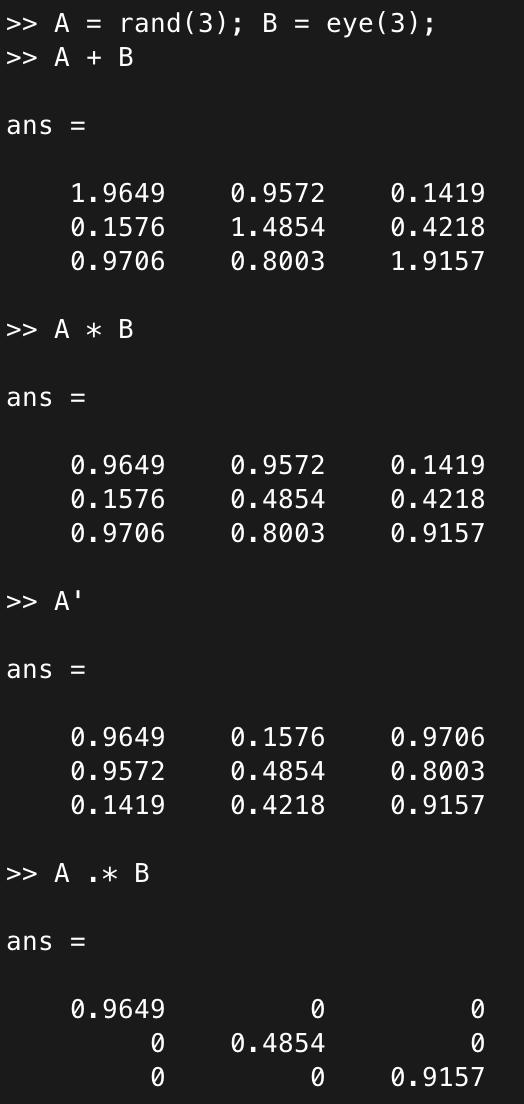
\includegraphics[width=\textwidth]{fig/matlab_mo}
	\end{minipage}
	\begin{minipage}{0.53\textwidth}
		\centering
		Python\\
		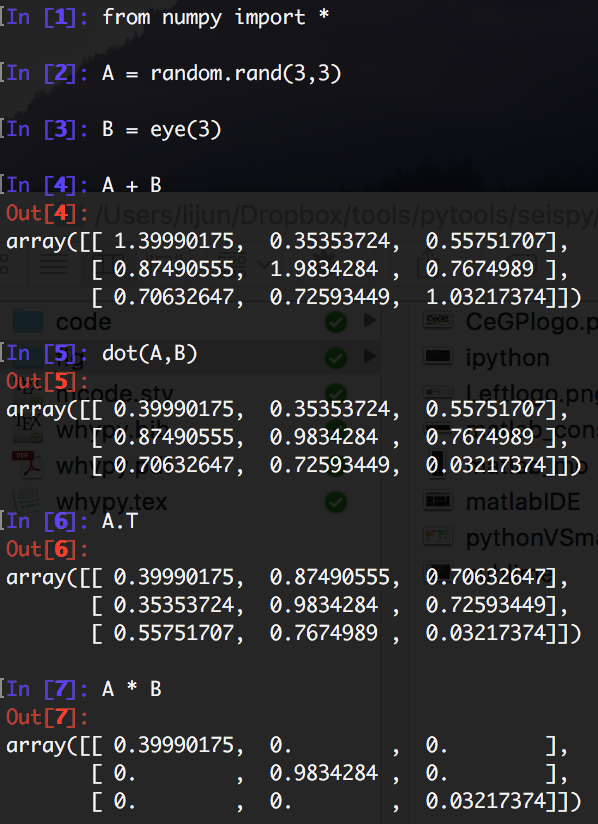
\includegraphics[width=\textwidth]{fig/python_mo}
	\end{minipage}
\end{frame}

\begin{frame}
	\frametitle{Linear algebra}
	\centering
	\begin{minipage}{0.35\textwidth}
		\centering
		MATLAB\\
		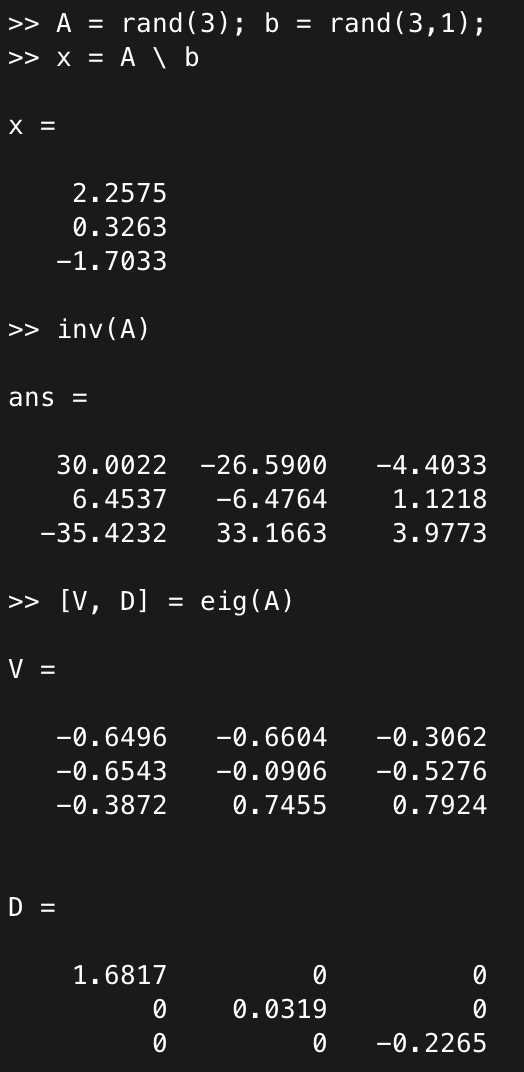
\includegraphics[width=\textwidth]{fig/matlab_la}
	\end{minipage}
	\begin{minipage}{0.53\textwidth}
		\centering
		Python\\
		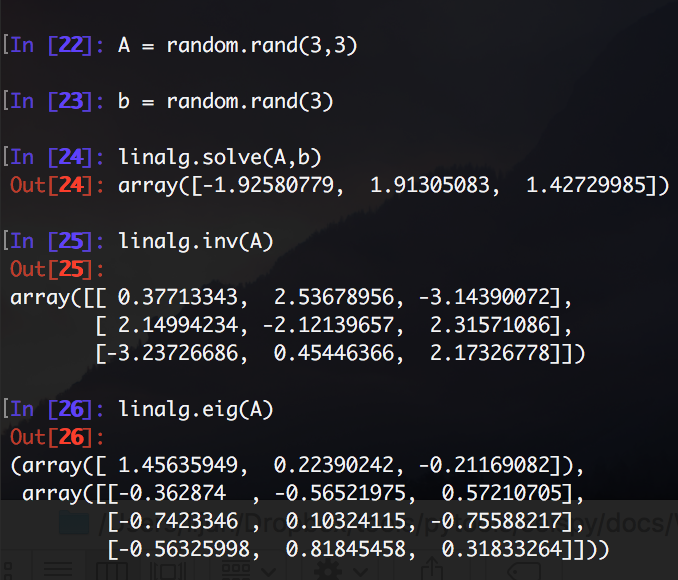
\includegraphics[width=\textwidth]{fig/python_la}
	\end{minipage}
\end{frame}

\begin{frame}
	\frametitle{Plotting(MATLAB)}
	\centering
	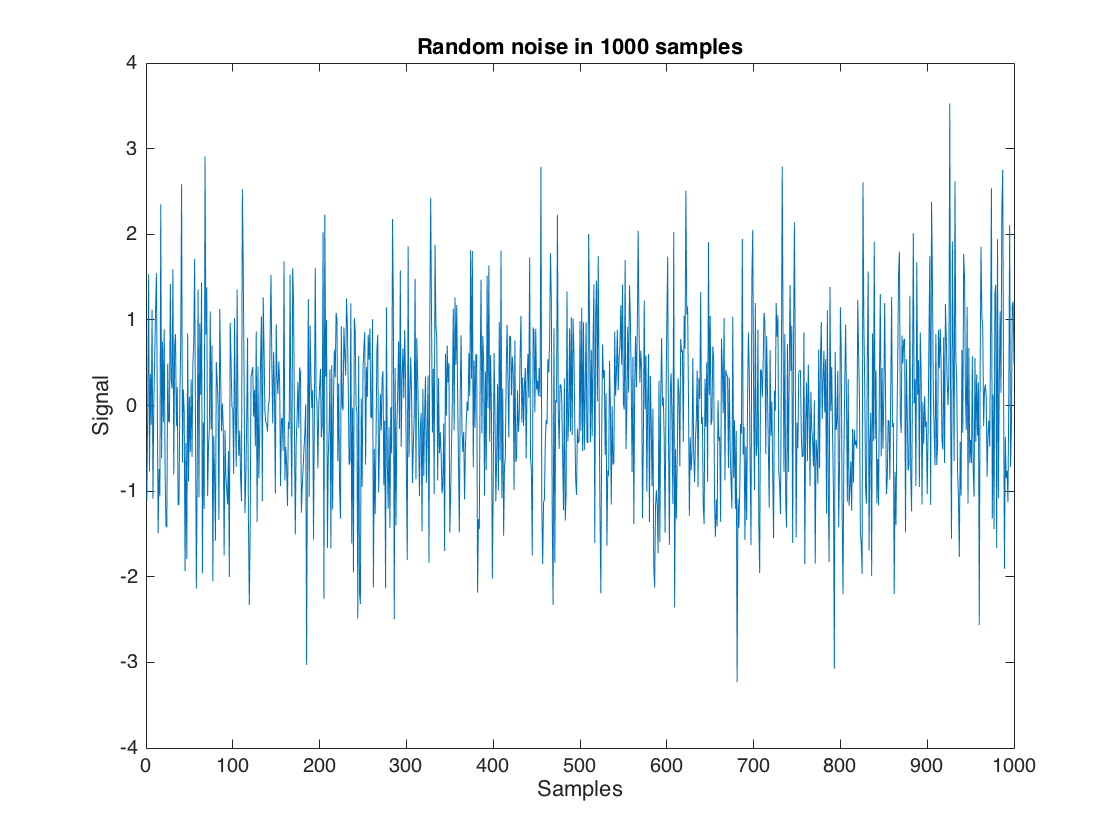
\includegraphics[width=\textwidth]{fig/matlab_plot}
\end{frame}

\begin{frame}
	\frametitle{Plotting(Python)}
	\centering
	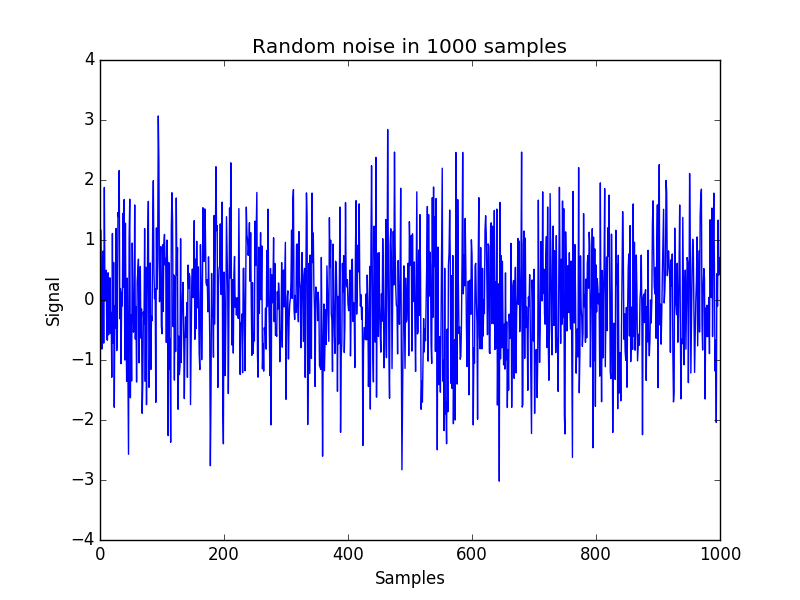
\includegraphics[width=\textwidth]{fig/python_plot}
\end{frame}

\begin{frame}
	\frametitle{Signal Processing}
	\centering
	MATLAB:\\
	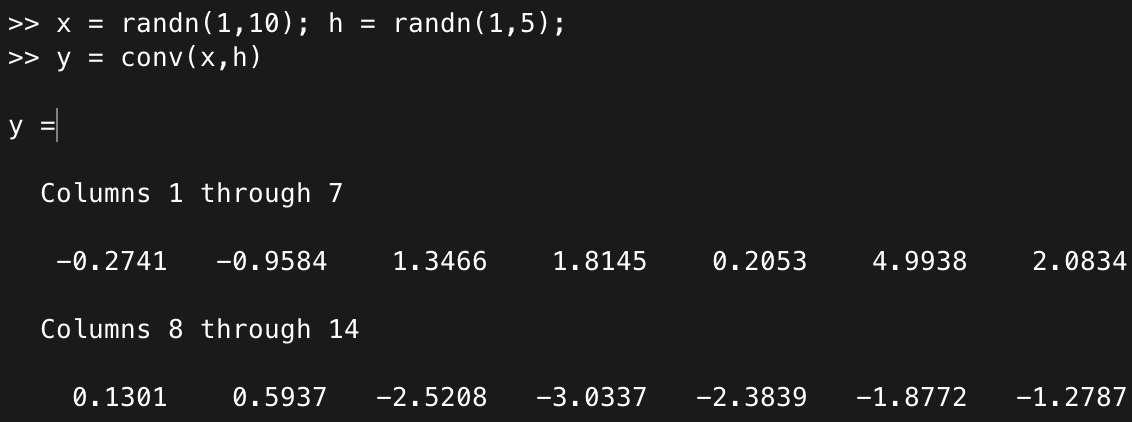
\includegraphics[width=0.9\textwidth]{fig/matlab_sp}\\
	Python:\\
	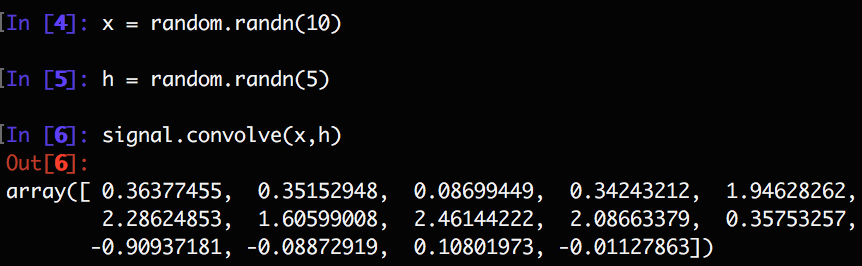
\includegraphics[width=0.9\textwidth]{fig/python_sp}	
\end{frame}

\begin{frame}
	\frametitle{Optimization}
	\begin{itemize}
		\item Find the minima of multi-dimensional Rosenbrock function
		\item MATLAB:
		\lstinputlisting[firstline=11,lastline=20]{code/demo.m}
		\item Python:
		\lstinputlisting[language=Python, firstline=11,lastline=20]{code/demo.py}
	\end{itemize}
\end{frame}

\begin{frame}
	\frametitle{Summary: features}
	\begin{itemize}
		\item Most MATLAB features has a corresponding package/module in Python
		\item Syntax of MATLAB and Numpy/Scipy are similar: 
		\begin{itemize}
			\item MATLAB syntax may be native to \textcolor{red}{matrix operation}
			\item Python syntax is more similar to other \textcolor{red}{programming language}
		\end{itemize}
		\item There is little thing in MATLAB that I cannot do in Python
	\end{itemize}
\end{frame}

\subsection{Performance}
\begin{frame}
	\frametitle{Performance comparison between MATLAB and Numpy/Scipy}
	\begin{table}
		%\caption{Performance between MATLAB and Numpy/Scipy}
		\begin{tabular}{|l|c|c|}
			\hline
			Items($1000\times1000$, sec) & MATLAB & Numpy/Scipy\\\hline
			Random matrix			& 	1.43000e-02 	& 	3.53193e-02\\\hline
			Matrix summation		&	6.03940e-04 	&	1.14631e-03\\\hline
			Matrix inverse			&	2.58000e-02		&	3.14017e-02\\\hline
			Matrix transpose		&	1.50000e-03		&	\textcolor{green}{7.28061e-07}\\\hline
			Matrix multiply			&	1.34000e-02		&	1.60881e-02\\\hline
			Solving linear system	&	1.41000e-02		&	1.63246e-02\\\hline
			Determinant				&	8.60000e-03		&	1.67287e-02\\\hline
			Norm						&	4.60000e-03		&	\textcolor{red}{1.64028e-02}\\\hline
			Eigenvalue Decompose	&	1.28600e+00		&	1.35907e+00\\\hline
			SVD						&	3.63800e-01		&	4.51565e-01\\\hline
			FFT						&	9.75997e-06		&	3.64929e-05/1.59512e-05\\\hline
			Spectrogram				&	4.62803e-03		&	\textcolor{green}{2.55447e-03}\\\hline
		\end{tabular}
	\end{table}
	\begin{itemize}
		\tiny
		\item MATLAB comes Intel MKL hardware acceleration while Numpy/Scipy requires additional config/compilation (not included in above table)
		%\item Numpy/Scipy use fftpack instead of fftw due to license issues.
	\end{itemize}
\end{frame}

\begin{frame}
	\frametitle{Performance between MATLAB and Numpy/Scipy (cont.)}
	\begin{itemize}
		\item In general, MATLAB(w/ MKL) is \textcolor{red}{faster}(no more than twice) than Numpy/Scipy(w/o MKL)
		\item Numpy/Scipy use fftpack instead of fftw due to license issues
		\item Numpy/Scipy matrix \textcolor{red}{transpose is significantly faster} than MATLAB due to data structure design; reason of slower norm is unknown
		\item Surprisingly, \textcolor{red}{spectrogram is faster} in Numpy/Scipy consider FFT has the opposite results
		\vspace{1cm}
		\item In conclusion, Numpy/Scipy has comparable performance as MATLAB. Further optimization can be included if needed.
	\end{itemize}
\end{frame}

\begin{frame}
	\frametitle{Case study: fast wiggle plot for large seismic dataset}
	\begin{itemize}
		\item Demo \pause
		\item MATLAB has better performance than Matplotlib \pause
		\item Use PyQtGraph as an interface to Qt tools to optimize the graphic rendering \pause
		\item The graphic rendering is faster, but background computation is slower than MATLAB (room to continue improve) \pause
		\item Convert this wiggle() into a class to make passing options easier
	\end{itemize}
\end{frame}

\section{Python\textsuperscript{\texttrademark}'s advantage and downside}
\subsection{Python is more popular and available}
\begin{frame}
	\frametitle{Popularity: TIOBE Programming Community Index}
	\centering
	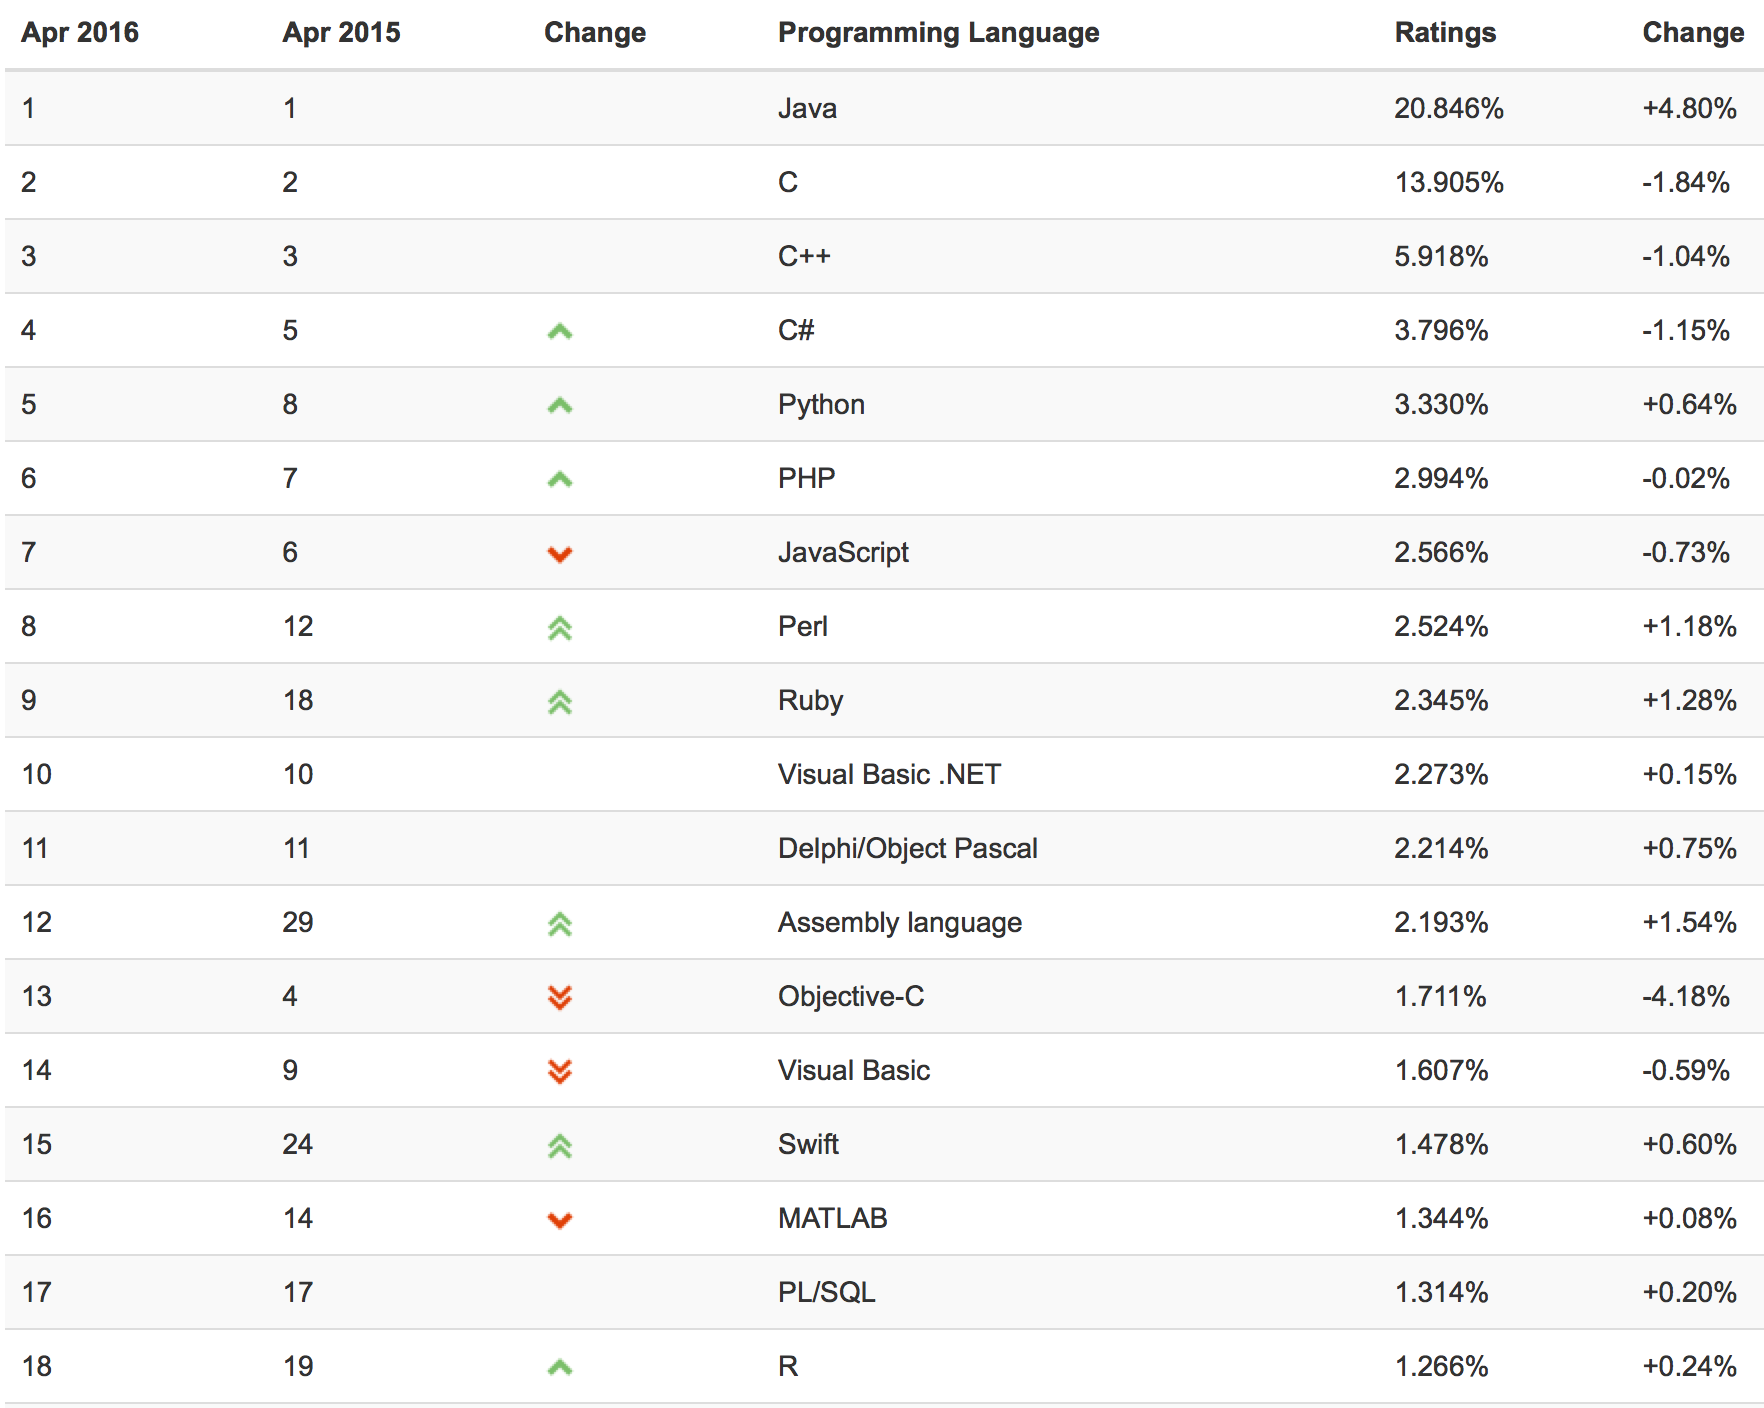
\includegraphics[width=0.9\textwidth]{fig/TIOBE}
\end{frame}

\begin{frame}
	\frametitle{Popularity: PYPL}
	\centering
	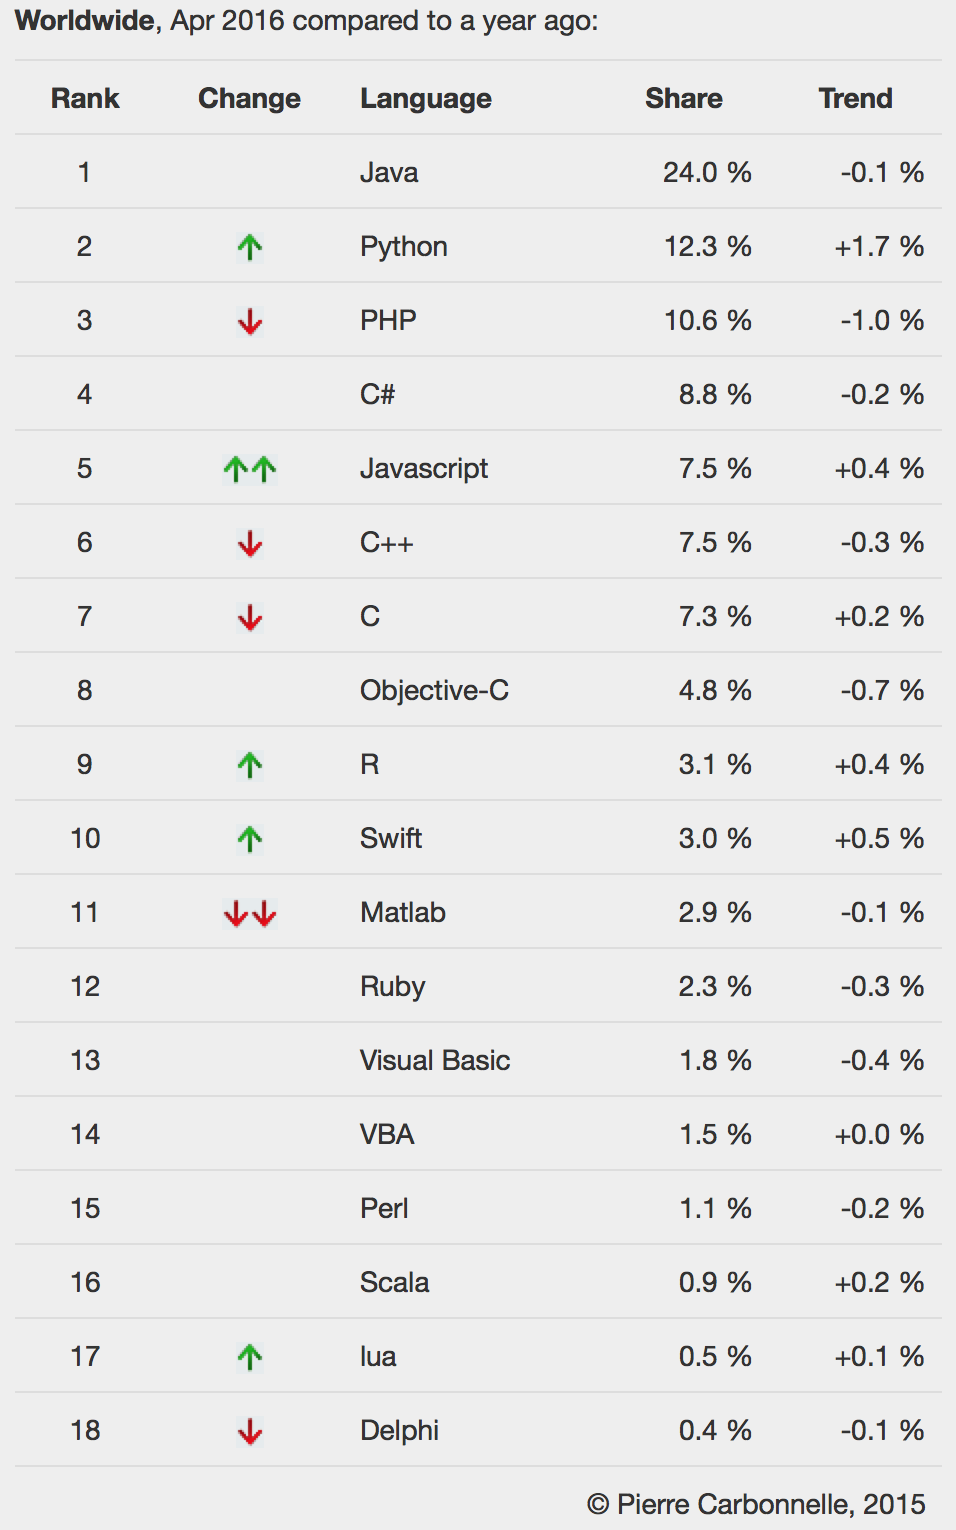
\includegraphics[width=0.35\textwidth]{fig/PYPL}
	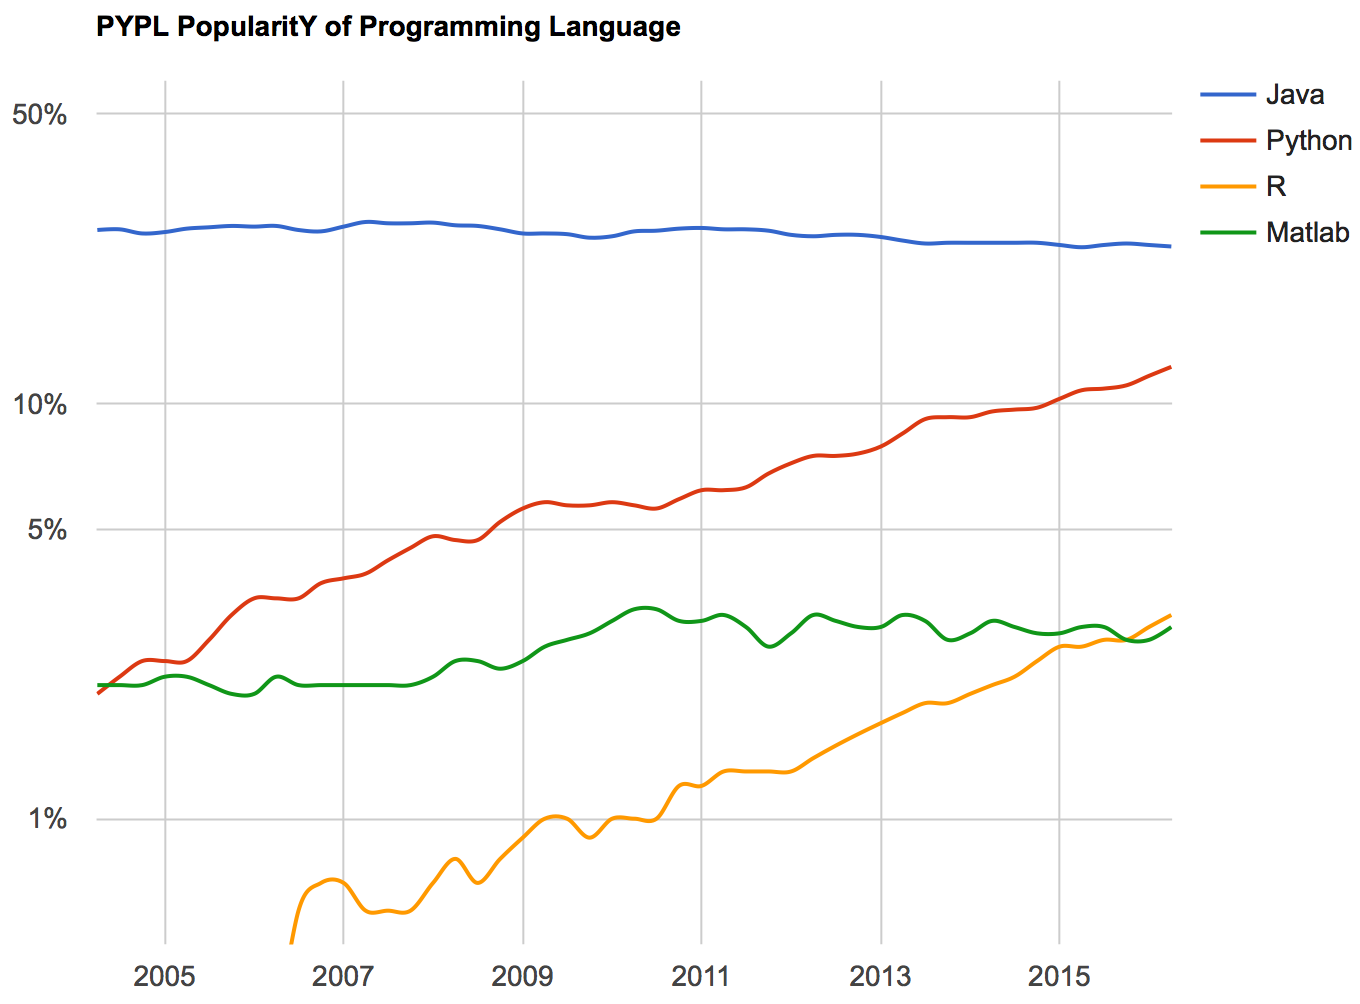
\includegraphics[width=0.7\textwidth]{fig/PYPL_trend}
\end{frame}

\begin{frame}
	\frametitle{Popularity: RedMonk Programming Language Rankings}
	\centering
	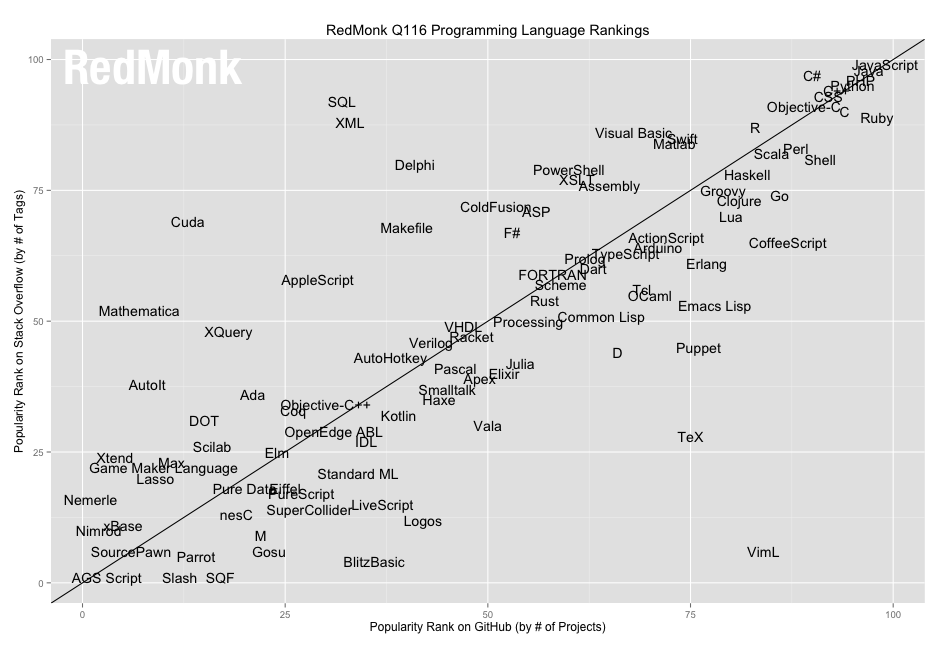
\includegraphics[width=1.05\textwidth]{fig/redmonk}
\end{frame}

\begin{frame}
	\frametitle{Availability and compatibility}
	\begin{itemize}
		\item Shortcomings of MATLAB\textsuperscript{\textregistered}
		\begin{itemize}
			\item Commercial software package (\textcolor{red}{proprietary} and can be \textcolor{red}{expensive}; but professionally \textcolor{red}{maintained and optimized})
			\item Implementation for functions/modules changes over different versions. \textcolor{red}{Tough backward compatibility}
			\item Porting can be \textcolor{red}{troublesome} (MCR requires exact same version installed); MATLAB behaves a little different between Windows and Un*x
		\end{itemize}
		\item How Python\textsuperscript{\texttrademark} fixes them
		\begin{itemize}
			\item \textcolor{red}{Open source} and \textcolor{red}{free} (personal and commercial use)
			\item Community developed and maintained, \textcolor{red}{possible bugs}
			\item Dedicated tools to even the gap between v.2 and v.3
			\item ALMOST \textcolor{red}{platform independent}
			\item \textcolor{red}{Virtual environment} is ideal for porting and collaboration 
		\end{itemize}
	\end{itemize}
\end{frame}

\subsection{Programming in Python feels natural and convenient}
\begin{frame}
	\frametitle{Programming language}
	\begin{itemize}
		\item Language wise
		\begin{itemize}
			\item MATLAB is historically a \textcolor{red}{wrapper} around LA/SP tools developed in C/Fortran. It's \textcolor{red}{evolving into} a \textcolor{red}{programming language}
			\item Python is a high-level, general-purpose, interpreted, dynamic \textcolor{red}{programming language}. It can be \textcolor{red}{used in scientific computing}
		\end{itemize}
		\item \textcolor{red}{Object-oriented} programming is natural in Python while can be awkward sometimes in MATLAB
		\item Functions in scripts are allowed Python but not MATLAB. Much \textcolor{red}{few files} to keep in development and \textcolor{red}{better project structure}.
		\item Data structure wise
		\begin{itemize}
			\item MATLAB: array, cell, structure; matrix based computation
			\item Python: list, set, dict, tuple; generator based computation 
		\end{itemize}
	\end{itemize}
\end{frame}


\begin{frame}
	\frametitle{Readability}
	\begin{itemize}
		\item MATLAB:
		\lstinputlisting[firstline=1, lastline=5]{code/demo.m}
		\item Python:
		\lstinputlisting[language=Python, firstline=1, lastline=4]{code/demo.py}
	\end{itemize}
\end{frame}

\begin{frame}
	\frametitle{Readability (cont.)}
	\begin{itemize}
		\item MATLAB is more intuitive for linear algebra operations
		\item MATLAB:
		\lstinputlisting[firstline=21, lastline=30]{code/demo.m}
		\item Python:
		\lstinputlisting[language=Python, firstline=31, lastline=40]{code/demo.py}
	\end{itemize}
\end{frame}

\begin{frame}
	\frametitle{Readability (cont.)}
	\begin{itemize}
		\item Python allow function definition in a script/module
		\lstinputlisting[language=Python, firstline=21, lastline=30]{code/demo.py}
		\item Those functions are usable from ``Import'' and make code generally more compact and orgainized
		\item Matlab requires lots of small files for function definition which propose ``copy and paste'' programming
	\end{itemize}
\end{frame}

\begin{frame}
	\frametitle{Balance of High Level and Low Level Programming}
	\begin{itemize}
		\item Use Cython to convert python module to C code (Demo) \pause
		\item Use Python C/\CC API to import complete C/\CC code or library (like MEX in MATLAB)
	\end{itemize}
\end{frame}

\begin{frame}
	\frametitle{Test frame work}
	\lstinputlisting[language=Python,firstline=1,lastline=18]{code/ut_example.py}
\end{frame}

\begin{frame}
	\frametitle{Online resource and document}
	\begin{itemize}
		\item \href{http://www.mathworks.com/matlabcentral/fileexchange/?s_tid=gn_mlc_fx}{File Exchange} vs. \href{https://pypi.python.org/pypi}{PyPI}
		\item List of functions (\href{http://www.mathworks.com/matlabcentral/fileexchange/56623-hyperplot-tools}{Hyperplot Tools}) vs. Online documentation (\href{http://www.pyqtgraph.org/}{PyQtGraph})
		\item Software install/update: Manually download vs \href{https://pypi.python.org/pypi/pip}{pip}
		\item Fragmental(MATLAB) vs centric(Python) package search experience
		\item Standard project and package system(\href{https://github.com/audreyr/cookiecutter}{Cookiecutter}) with integration of Github, GitFlow, Sphinx, and PyPI
	\end{itemize}
\end{frame}

\begin{frame}
	\frametitle{Downsides of Python}
	\begin{itemize}
		\item Too many choices for packages, difficult to choose (ironic, but true)
		\item Many scientific computing packages are developed and distributed in MATLAB
		\item Good news: they can be ported to Python
		\begin{itemize}
			\item CVX: \href{http://cvxopt.org/}{CVXOPT}
			\item SPGL1: \href{https://github.com/drrelyea/SPGL1\_python\_port}{SPGL1\_python\_port}
		\end{itemize}
	\end{itemize}
\end{frame}



\section{Useful packages for Python}
\begin{frame}
	\frametitle{Useful packages for Python}
	\begin{itemize}
		\item Python comes with a very small set of built-in module for basic operation and file handling
		\item Packages must-have for scientific computing
		\begin{itemize}
			\item \href{http://www.numpy.org/}{Numpy} for matrix operation
			\item \href{https://www.scipy.org/}{Scipy} for linear algebra, signal processing, optimization and etc.
			\item \href{http://matplotlib.org/}{Matplotlib} for 2D plot
		\end{itemize}
		\item Packages recommended for trying
		\begin{itemize}
			\item \href{https://hgomersall.github.io/pyFFTW/}{pyFFTW} for fast Fourier Transform
			\item \href{https://stanford.edu/~mwaskom/software/seaborn/}{Seabron} for statistical data visuallization
			\item \href{http://www.pyqtgraph.org/}{PyQtGraph} for scientific graphics and GUI library to generate fast and interactive plots
			\item \href{http://www.sagemath.org/}{SAGE} aims to be a replacement for MATLAB
			\item \href{https://github.com/obspy/obspy/wiki}{ObsPy} is a Python framework for seismology (segy, sac i/o)
			\item \href{http://scikit-learn.org/stable/}{scikit-learn} for machine learning 
		\end{itemize}
	\end{itemize}
\end{frame}

\begin{frame}
	\frametitle{ObsPy}
	\begin{itemize}
		\item ObsPy is an open-source project dedicated to provide a Python framework for processing seismological data.
		\item Handles a good variety of file types and databases with a large \href{https://docs.obspy.org/packages/index.html}{library}
		\item Generate standard \href{https://docs.obspy.org/gallery.html}{plots} for natural earthquake publication 
	\end{itemize}
\end{frame}

\begin{frame}
	\frametitle{Seaborn}
	\begin{itemize}
		\item Excellent lib for 2D plot of statistical data
		\item Most types of \href{https://stanford.edu/~mwaskom/software/seaborn/examples/index.html}{plot} you can think of
		\item Easy \href{https://stanford.edu/~mwaskom/software/seaborn/installing.html}{install} and setup
	\end{itemize}
\end{frame}

\begin{frame}
	\frametitle{SageMath}
	\begin{itemize}
		\item Their \href{http://www.sagemath.org/}{mission}: create a viable free open source alternative to Magma, Maple, Mathematica and Matlab
		\item Popular in some mathematical area
		\item Includes: NumPy, SciPy, matplotlib, Sympy, Maxima, GAP, FLINT, R etc.
	\end{itemize}
\end{frame}

\begin{frame}
	\frametitle{scikit-learn}
	\begin{itemize}
		\item A great easy-to-start machine learning \href{http://scikit-learn.org/stable/index.html}{framework} in Python
		\item Includes \href{http://scikit-learn.org/stable/user\_guide.html}{common methods} for supervised learning, unsupervised learning, model selection etc. 
		\item Good material for learning those ML algorithms.
	\end{itemize}
\end{frame}

\begin{frame}
	\frametitle{scikit-learn}
	\centering
	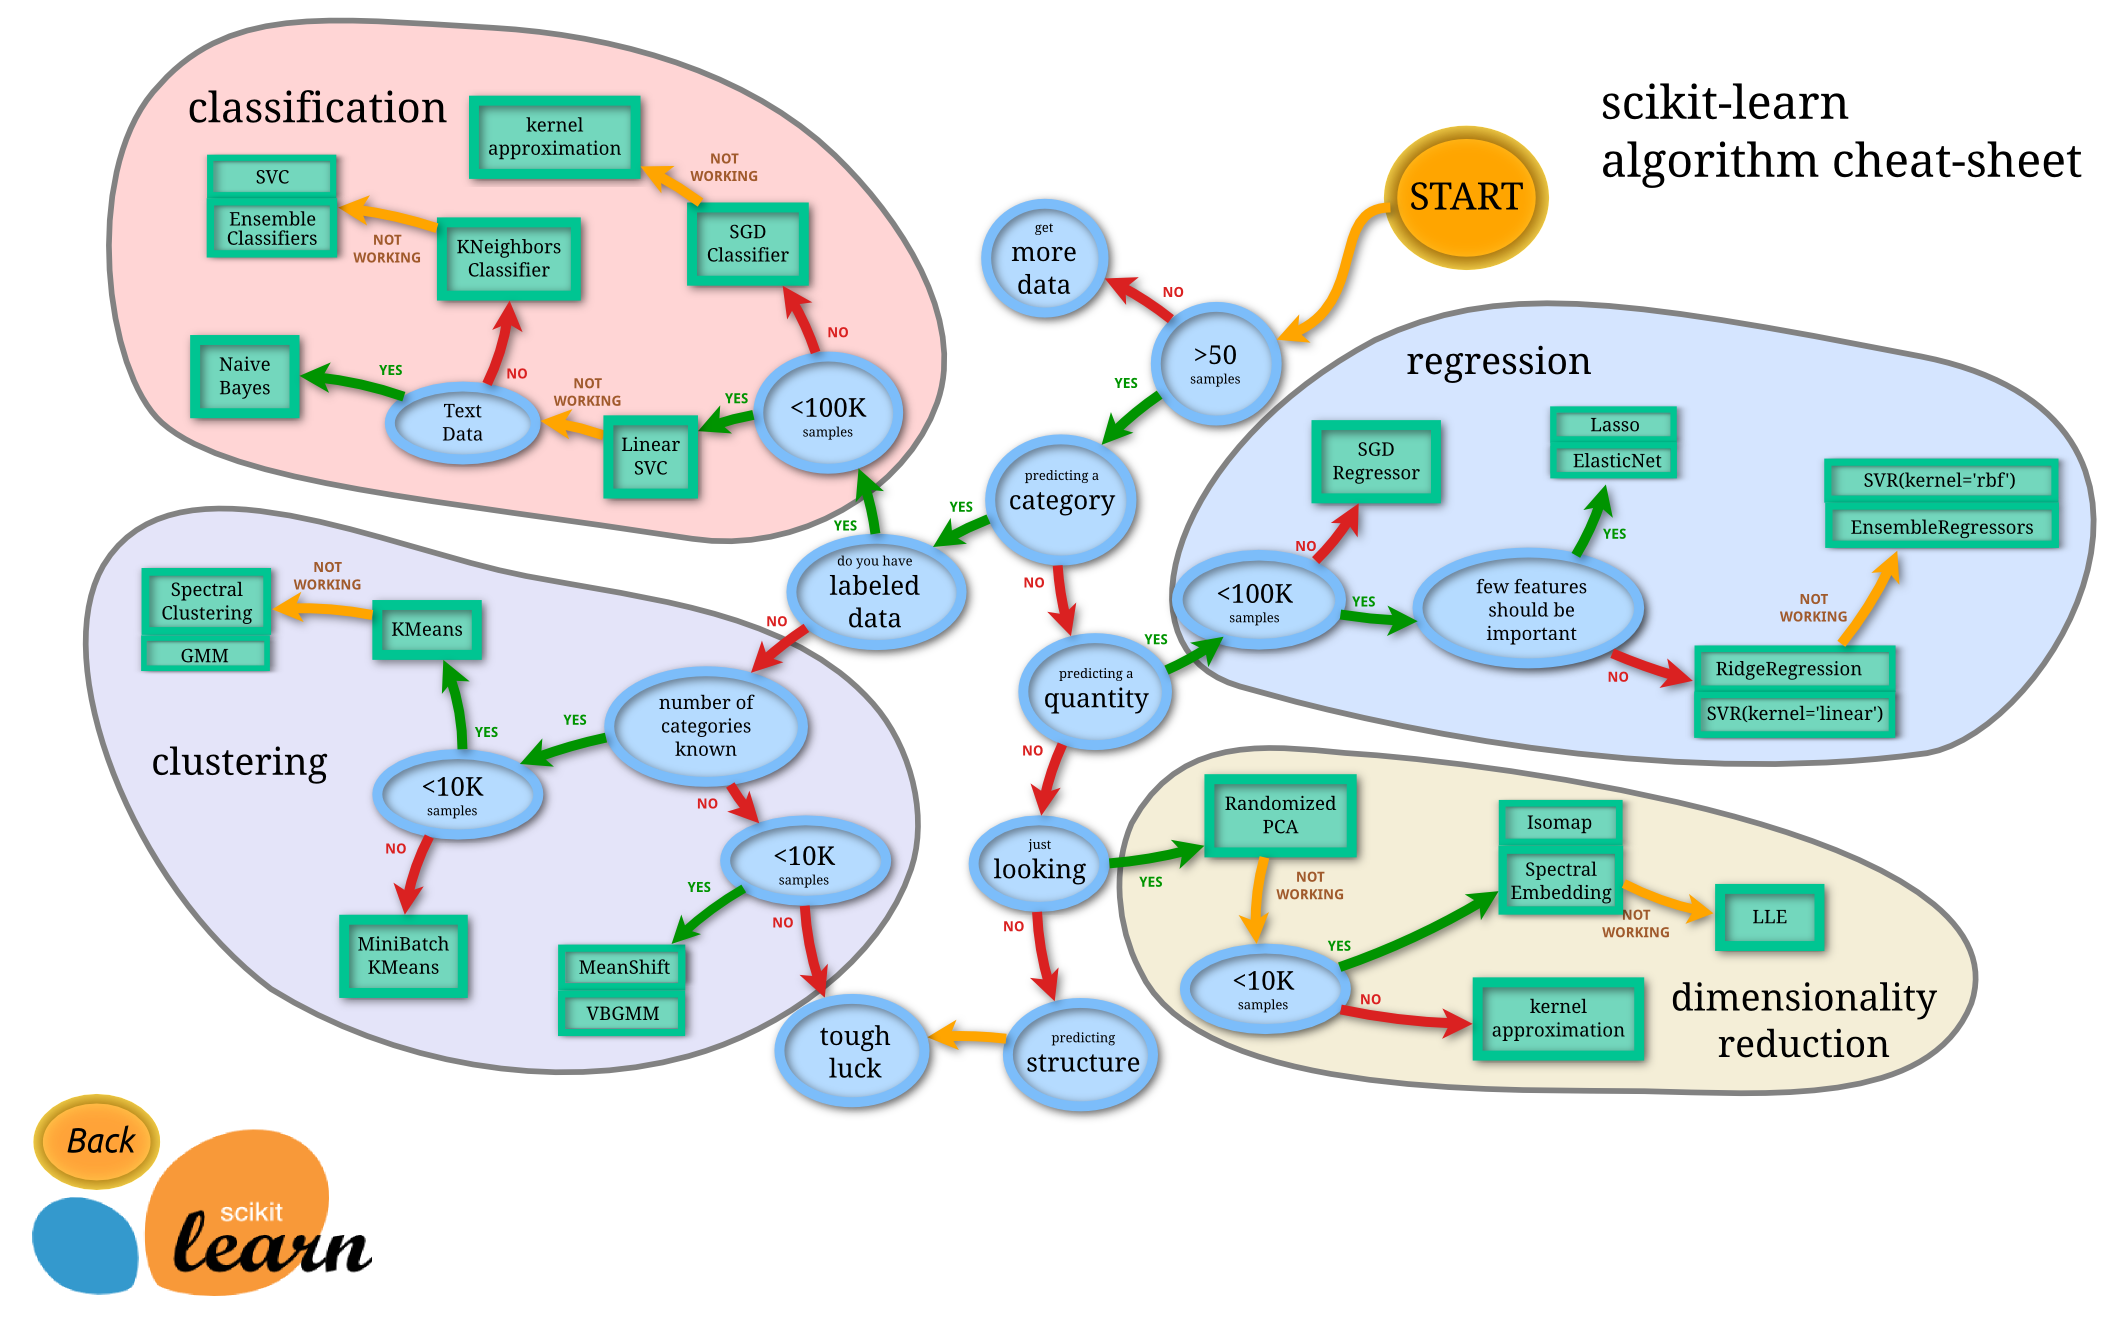
\includegraphics[width=1.1\textwidth]{fig/ml_map}
\end{frame}

\begin{frame}
	\frametitle{OpenCV-Python}
	\begin{itemize}
		\item \href{http://docs.opencv.org/3.1.0/d0/de3/tutorial\_py\_intro.html\#gsc.tab=0}{OpenCV-Python} is a library of Python bindings designed to solve computer vision problems
		\item OpenCV-Python is a Python wrapper for the original OpenCV C++ implementation
		\item OpenCV-Python makes use of Numpy and can be easily integrated with SciPy and Matplotlib.
	\end{itemize}
\end{frame}

\begin{frame}
	\frametitle{Complete programming solution + full-functional playground}
	\begin{itemize}
		\item MATLAB has a mature IDE with sweet number of packages
		\item MATLAB is optimized for matrix operation and is ideal to test the water for new algorithms (Fancy scientific calculator with programming functionality)
		\vspace{1cm}
		\item Python is more versatile with reasonable performance %(In every fields that Python works, you may be able to find a better one. But Python always comes the second/third place)
		\item Python packages are easy to develop, deploy and maintain
		\vspace{1cm}
		\item I see a future that using Python as the main development tools while keep MATLAB as a playground for quick algorithm verification
	\end{itemize}
\end{frame}

% Reference
%\begin{frame}%[allowframebreaks] %in case more than 1 slide needed
%	\frametitle{References}
%	\footnotesize
%	\bibliographystyle{seg}
%	\bibliography{whypy}
%\end{frame}

\begin{frame}
	\frametitle{Reference: Python/MATLAB comparison}
	\begin{itemize}
		\item \href{http://cyrille.rossant.net/why-using-python-for-scientific-computing/}{Cyrille Rossant: Why use Python for scientific computing?}
		\item \href{https://sites.google.com/site/pythonforscientists/python-vs-matlab}{Almar Klein: Python vs Matlab}
	    \item \href{https://stevetjoa.com/305/}{Steve Tjoa: I used Matlab. Now I use Python.}
    	\item \href{http://phillipmfeldman.org/Python/Advantages_of_Python_Over_Matlab.html}{Philippe Feldman: Eight Advantages of Python Over Matlab}
    	\item \href{https://vnoel.wordpress.com/2008/05/03/bye-matlab-hello-python-thanks-sage/}{Vincent Noël: Bye Matlab, hello Python, thanks Sage}
    	\item \href{http://www.stat.washington.edu/~hoytak/blog/whypython.html}{Hoyt Koepke: 10 Reasons Python Rocks for Research (And a Few Reasons it Doesn’t)}
	\end{itemize}
\end{frame}

\begin{frame}
	\frametitle{\hypertarget{ref:SAC}{IRIS database and SAC tools}}
	\begin{itemize}
		\item \href{https://ds.iris.edu/ds/nodes/dmc/software/downloads/sac/}{IRIS DMC: (SAC) a general purpose interactive program designed for the study of sequential signals, especially time series dat}
		\item \href{http://ds.iris.edu/ds/nodes/dmc/software/downloads/irisfetch.m/}{IRIS DMC: (irisFetch.m) the Matlab library IRISFETCH allows seamless access to data stored within the IRIS-DMC}
		\item \href{http://geophysics.eas.gatech.edu/people/zpeng/Teaching/SAC_Tutorial/\#part2_6}{Zhigang Peng: (MatSAC) Read/Write/Plot seismic data in SAC }
	\end{itemize}
\end{frame}

% Final slides
\begin{frame}
	\frametitle{Questions?}
	\begin{itemize}
		\Large \item Thanks for your attention!
		\vspace*{3cm}
		\tiny \item This work is supported by the Center for Energy and Geo
Processing (CeGP) at Georgia Tech and by King Fahd University
of Petroleum and Minerals (KFUPM).
	\end{itemize}
\end{frame}

\end{document}
